%\documentclass[titlepage,12pt,a4]{report}
%\documentclass[a4paper,10pt,titlepage]{article}
\documentclass[journal]{IEEEtran/IEEEtran}
\usepackage[utf8]{inputenc}
\usepackage{url}
\usepackage[colorlinks=true]{hyperref}
%\usepackage{todonotes}
\usepackage{color}
\usepackage{listings}
%\usepackage{mips_modified}
%\usepackage[titletoc]{appendix}
\usepackage{pdfpages}
\usepackage{caption,subcaption}	% package for making several pictures in one
\usepackage{float}				% package for restricting pictures to float about (use: \begin{figure}[H])
\usepackage{graphicx}
%\usepackage{multirow}			% package for multirow and multicolumn tables
\definecolor{dkgreen}{rgb}{0,0.6,0}
\definecolor{gray}{rgb}{0.5,0.5,0.5}
\definecolor{mauve}{rgb}{0.58,0,0.82}

\lstset{ 				% must add \usepackage{listings}
%  language=VHDL,			% the language of the code
  language=C++,
%  language={[mips]Assembler},
%  columns=flexible,
%  keepspaces=true,
  basicstyle=\footnotesize,	% the size of the fonts that are used for the code
  numbers=left,			% where to put the line-numbers
  numberstyle=\tiny\color{gray},	% the style that is used for the line-numbers
  stepnumber=1,			% the step between two line-numbers. If it's 1, each line will be numbered
  numbersep=5pt,			% how far the line-numbers are from the code
  backgroundcolor=\color{white},% choose the background color. You must add \usepackage{color}
  showspaces=false,		% show spaces adding particular underscores
  showstringspaces=false,		% underline spaces within strings
  showtabs=false,			% show tabs within strings adding particular underscores
  frame=l,				% adds a frame around the code
  rulecolor=\color{black},		% if not set, the frame-color may be changed on line-breaks within not-black text (e.g. commens (green here))
  tabsize=4,				% sets default tabsize to 2 spaces
  captionpos=b,			% sets the caption-position to bottom
  breaklines=true,			% sets automatic line breaking
  breakatwhitespace=false,	% sets if automatic breaks should only happen at whitespace
  title=\lstname,			% show the filename of files included with \lstinputlisting; also try caption instead of title
  keywordstyle=\color{blue},	% keyword style
  commentstyle=\color{dkgreen},% comment style
  stringstyle=\color{mauve},	% string literal style
  escapeinside={\%*}{*)},	% if you want to add a comment within your code
  morekeywords={*,...}		% if you want to add more keywords to the set
}

\title{TDT4260 Miniproject---Prefetching Strategies}
%dTDT4260 Supadupah prefetchahz}
\author{Joakim E.C. Andersson \and Jakob D. Knutsen \and Håkon F. Amundsen \and Benjamin Bjørnseth}
\begin{document}

\maketitle

% ToC looks a bit messy, and maybe not necessary for our small report?
%\tableofcontents

% Evaluation criterion:
%- Language and use of figures
%- Clarity of the problem statement
%- Overall document structure
%- Depth of understanding for the field of computer architecture
%- Depth of understanding of the investigated problem

% Using input instead of include removes the \newpage, which would
% make our report too long!
% Evaluation criterion:
%- Language and use of figures
%- Clarity of the problem statement
%- Overall document structure
%- Depth of understanding for the field of computer architecture
%- Depth of understanding of the investigated problem

\begin{abstract}
%  Short description of what the context of the report is (maybe?), the
%  work we are describing in this report, and what our results are.
  
  In this paper, we investigate the relationship between different
  prefetching strategies and speedups in a suite of different programs
  from the SPEC CPU2000 benchmark. We do this by implementing and
  running the prefetching strategies for an L2 cache using the M5
  simulator. We do not yet know what we discover!

\end{abstract}
% Evaluation criterion:
%- Language and use of figures
%- Clarity of the problem statement
%- Overall document structure
%- Depth of understanding for the field of computer architecture
%- Depth of understanding of the investigated problem

\section{Introduction}
\label{sec:introduction}
Over the last 3 decades, processor performance has increased more than memory performance,
which has led to what is commonly known as the Memory Gap (see figure~\ref{img:mem_gap}). In order to remedy this, a memory
hierarchy is used to provide the illusion of a very fast and very
large memory (see figure~\ref{img:mem_hier}). 

\begin{figure}[H]
	\centering
	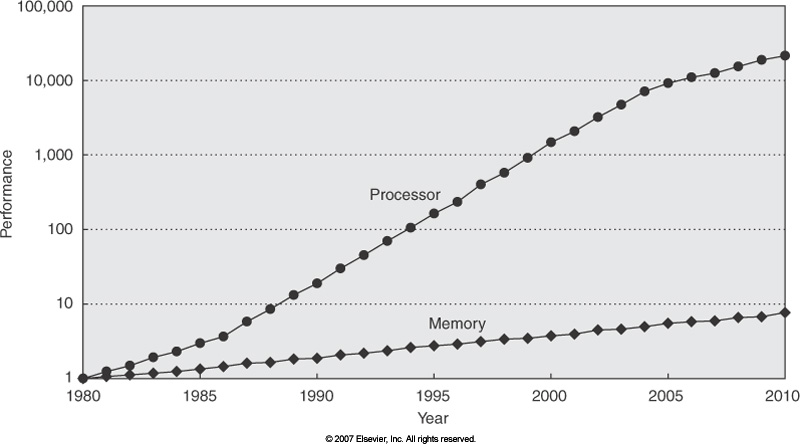
\includegraphics[scale=0.3]{./img/mem_gap}
	\caption{The memory gap}
	\label{img:mem_gap}
\end{figure}

The illusion will only partially hold, however, as the processor is
delayed for the entire main memory access time when the memory contents required
is not present in any of the caches. One technique
which has been introduced in order to face this problem is prefetching. Prefetching improves the utilization of the caches. This technique
attempts to improve the cache hit rate by predicting what memory
addresses the processor will want to access in the near future, and
issuing fetches from the main memory before the processor actually
needs the contents so that the data will reside in cache when the
processor does require it. This is usually accomplished by recording
memory access history and statistics, and using this to make educated
guesses about the future. 
{\bf (references, citations)}

\begin{figure}[H]
	\centering
	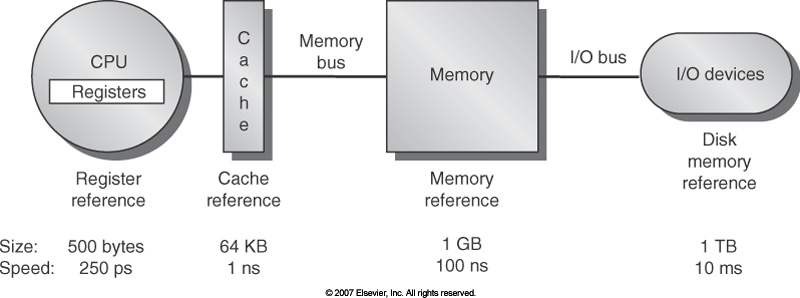
\includegraphics[scale=0.3]{./img/mem_hier}
	\caption{The memory hierarchy}
	\label{img:mem_hier}
\end{figure}

In this paper, we are going to investigate how different kinds of
prefetching strategies affects the efficiency of the prefetcher when
run on several different programs from the SPEC CPU2000 benchmark
suite.  {\bf (references, citations)}

% Evaluation criterion:
%- Language and use of figures
%- Clarity of the problem statement
%- Overall document structure
%- Depth of understanding for the field of computer architecture
%- Depth of understanding of the investigated problem

\section{Related Work}
\label{sec:relatedWork}

A large number of different prefetching strategies have been proposed,
with the intent of either being better at adapting to the needs of
different applications or recognizing an access pattern which is not
adequately handled in existing prefetchers \textbf{(citation
  needed)}. The main inspiration for our prefetcher implementations is
Grannæs' paper~\cite{Grannas}. In the background section of this
paper, Grannæs describes five different categories of hardware
prefetchers: sequential prefetchers, instruction based prefetchers,
address based prefetchers, spatial locality prefetchers and linked
data prefetchers. Several examples of the different types of
prefetchers are given, with references to articles discussing some of
the different kinds in more detail.  {\bf (references, citations)}
 % May also be called "background"
% Evaluation criterion:
%- Language and use of figures
%- Clarity of the problem statement
%- Overall document structure
%- Depth of understanding for the field of computer architecture
%- Depth of understanding of the investigated problem

\section{Prefetcher Description}
\label{sec:prefetcherDescription}

In our paper, we will consider four different prefetching strategies,
each taken from a separate category of prefetchers identified in
Grannas' paper (reference needed).

\subsection{Sequential Prefetcher}
\label{sec:sequentialPrefetcher}
The sequential prefetcher is based on the fact that memory accesses often follow a sequential pattern. When accessing the members of an array, or iterating through a loop, most of the memory accesses will follow a stride-n pattern (where n is the number of addresses between the accessed addressess). 

The sequential prefetcher keeps track of the last \emph{n} values, and also keeps track of for how long the current stride has been ongoing. The prefetchers agressiveness can be configured by configuring the amount of strides that needs to be discovered before the prefetcher will react on a memory access. 

For each memory access, the memory address is compared to the last memory address. If the current stride value corresponds to the difference, the number of current strides is updated. If the number of current strides is greater than or equal to the required/configured amunt of strides, a prefetched address is returned.
{\bf (references, citations)}

\subsection{Global History Buffer Prefetcher}
\label{sec:ghbPcdcPrefetcher}
The global history buffer prefetcher is an instruction based
prefetching scheme. In this schem, a datastrcture called Global
History Buffer (abbreviated GHB) is maintained. This datastructure is
a table which containsr  ... We implement a variety called GHB/PCDC (Global History
Buffer, Program Counter based with Delta Correlation).  {\bf
  (references, citations)}

\subsection{Markov Prefetcher}
\label{sec:markovPrefetcher}
The Markov prefetcher is an address based prefetcher,...
{\bf (references, citations)}

\subsection{Spatial Memory Streaming Prefetcher}
\label{sec:smsPrefetcher}
The Spatial Memory Streaming (SMS) Prefetcher is a spatial locality
prefetcher...  {\bf (references, citations)}
 % May rename this to something more appropriate
% Evaluation criterion:
%- Language and use of figures
%- Clarity of the problem statement
%- Overall document structure
%- Depth of understanding for the field of computer architecture
%- Depth of understanding of the investigated problem

\section{Methodology}
\label{sec:methodology}

To discover what the effect of using different prefetching strategies
for different applications are, we used a modified version of the M5
simulator, version 2.0 \cite{M5} as a testing platform. This simulator
is a software implementation loosely based on the Alpha 21264
processor\cite{Alpha}. The version used was provided by the course
staff, and included an interface to the L2 cache prefetching
functionality of the simulator. By using this interface, we could
integrate our prefetchers into the processor simulator, such that the
resulting binaries would be a simulator of the processor with a
specific prefetcher algorithm in control of prefetching for the L2 cache.

For each of the simulators built this way, we executed a suite of
programs from the SPEC CPU2000 benchmark. The programs used are listed
in table~\ref{tab:benchmarks}. The simulator software automatically
tracked key statistics during the program execution, such as cache
misses, prefetches issued, and clock cycles used for running the
program. By comparing the number of cycles used when executing the
program with our prefetchers included in the simulator to the number
of cycles used without a prefetcher, we could calculate the speedup due to the prefetcher for the different programs.

\begin{table}[htbp]
  \centering
  \begin{tabular}{|c|}
    \hline
    {\bf Benchmarks} \\ \hline
    ammp \\ \hline
    applu \\ \hline
    apsi \\ \hline
    art110 \\ \hline
    art470 \\ \hline
    bzip2\_graphic \\ \hline
    bzip2\_program \\ \hline
    bzip2\_source \\ \hline
    galgel \\ \hline
    swim \\ \hline
    twolf \\ \hline
    wupwise \\ \hline
  \end{tabular}
  \caption{The benchmarks used to evaluate the prefetcher efficiency.}
  \label{tab:benchmarks}
\end{table}

% Give prefetcher configurations
When implementing our prefetchers, there were a number of
implementation parameters which had to be set (e.g. the size of the
data structures used in the algorithm, the number of addresses to
prefetch). To get a fair comparisons between the different strategies,
we wanted to find the settings which yielded the highest average speedup for each
prefetcher. To make the prefetchers more realistic, we were only
allowed to use 8 KiB of storage internally in our prefetcher. This set
the bounds for our prefetcher configuration space. 

Our strategy for finding the optimal settings for the given prefetcher
was to set them initially to more or less arbitrary values within the
permissible range, and attempt to locate at least a local maximum by
varying the parameters in turn. Due to the enormous possible set of
values, only a few were tried for each degree of freedom---these are
listed in \autoref{tab:stridesettings}, \autoref{tab:ghbsettings},
\autoref{tab:smssettings} and \autoref{tab:markovsettings}. The
combination of parameters which yielded the highest average speedup
are marked in bold.

\begin{table}[htbp]
  \centering
  \begin{tabular}{|c|c|c|}
    \hline
    \textbf{Prefetch Degree} & \textbf{Consecutive strides} \\ \hline
    10 & 3 \\ \hline
    \textbf{15} & \textbf{4} \\ \hline
    15 & 5 \\ \hline % TODO: Not all these settings have been attempted yet...
  \end{tabular}
  \caption{The various parameters attempted for the ABSP. The prefetch degree is the number of consecutive blocks prefetched, the consecutive strides is how many consecutive constant step memory misses must occur before a prefetch is issued.}
  \label{tab:stridesettings}
\end{table}

\begin{table}[htbp]
  \centering
  \begin{tabular}{|c|c|}
    \hline
    \textbf{Table Size} & \textbf{Prefetch Degree} \\ \hline
    300 & 3 \\ \hline
    \textbf{350} & 5 \\ \hline
    400 & \textbf{10} \\ \hline
        & 15 \\ \hline
  \end{tabular}
  \caption{The various parameters attempted for the GHB/PCDC prefetcher. The table size is the number of entries in both the GHB and the index table---unequal sizes were not tested. The prefetch degree is the number of blocks to issue prefetches for, once you find a previous history match.}
  \label{tab:ghbsettings}
\end{table}

\begin{table}[htbp]
  \centering
  \begin{tabular}{|c|c|c|c|c|}
    \hline
    \textbf{Region (log2)} & \textbf{History Table} & \textbf{Filter Table} & \textbf{Accumulation Table} \\ \hline
    4  & 128 & 16 & 16 \\ \hline
    8  & \textbf{256} & 32&  \textbf{32}\\ \hline
    \textbf{11} &     & \textbf{64}&  64\\ \hline
  \end{tabular}
  \caption{The various parameters attempted for the SMS prefetcher.}
  \label{tab:smssettings}
\end{table}

\begin{table}[htbp]
  \centering
  \begin{tabular}{|c|c|}
    \hline
    \textbf{Table Size} & \textbf{Prefetch Degree} \\ \hline
    2000 & 2 \\ \hline
    4000 & 3 \\ \hline
    \textbf{6000} & \textbf{4} \\ \hline
  \end{tabular}
  \caption{The various parameters attempted for the Markov prefetcher. The table size is the maximum number of nodes in the Markov chain, and the prefetch degree is the number of edges to follow when prefetching.}
  \label{tab:markovsettings}
\end{table}


% \begin{table}[htbp]
%   \centering
%   \begin{tabular}{|c|c|}
%     \hline
%     \textbf{Prefetcher} & \textbf{Settings} \\ \hline
%     Stride & Wait for 4 consecutive strides, prefetch 15 blocks \\ \hline
%     GHB/PCDC & 350 entries in GHB and index table, prefetch 10 blocks  \\ \hline
%     SMS & \\ \hline
%     Markov & \\ \hline
%   \end{tabular}
%   \caption{The settings yielding optimal overall result for each prefetcher.}
%   \label{tab:settings}
% \end{table}


%Having  (... cannot remember what this was supposed to start :X)XS

% (should M5 description be in introduction?)

% (Should we say that they tests were run on a cluster?)  {\bf
% (references, citations)}

% Evaluation criterion:
%- Language and use of figures
%- Clarity of the problem statement
%- Overall document structure
%- Depth of understanding for the field of computer architecture
%- Depth of understanding of the investigated problem

\section{Result}
\label{sec:result}

The speedup from when running the selected applications with the
different prefetchers is tabulated in \autoref{fig:initResults}.

\begin{figure}[ht]
  \centering
  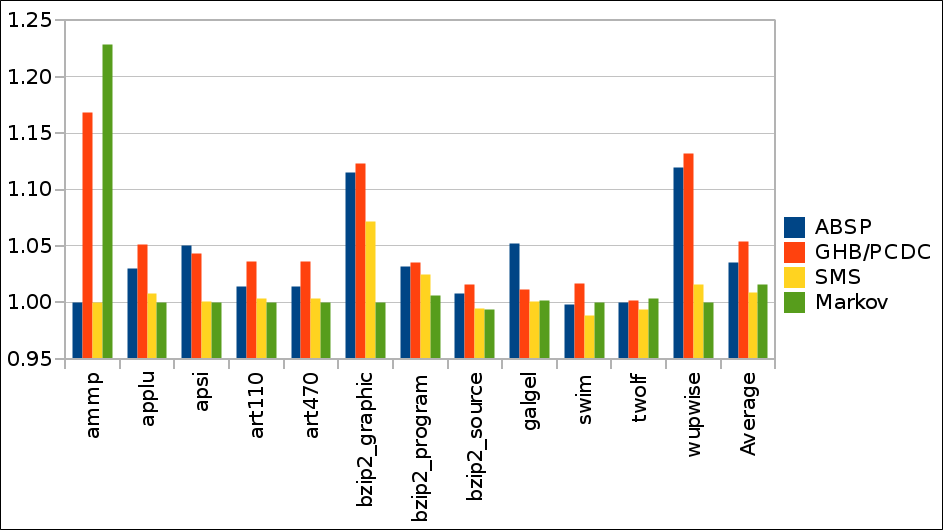
\includegraphics[scale=0.25]{figures/init_results.png}
  \caption{\label{fig:initResults} Speedup on the Y-axis plotted
    against program on the X-axis.}
\end{figure}

What other results? Should we include parameter search results? What
about results from experimenting with altering the prefetchers---does
that belong here or in the discussion section?XS

\subsection{Sequential Prefetcher Result}
\label{sec:sequentialPrefetcherResult}

\subsection{GHB Prefetcher Result}
\label{sec:ghbPrefetcherResult}

\subsection{Markov Prefetcher Result}
\label{sec:markovPrefetcherResult}

\subsection{Spatial Memory Streaming Prefetcher Result}
\label{sec:smsPrefetcherResult}


% Evaluation criterion:
%- Language and use of figures
%- Clarity of the problem statement
%- Overall document structure
%- Depth of understanding for the field of computer architecture
%- Depth of understanding of the investigated problem

\section{Discussion} % (fold)
\label{sec:discussion}

Can only be written when results are present.
Things to consider:

- How well do the different prefetchers perform on average?

- Are there any variance as to which programs they yield good speedup
on?

- How would combining them work?

- Considering how the time spent by our prefetching algorithms is not
taken into account, are our results at all accurate and usable?

- Anything else?

{\bf (references, citations)}

\section{Conclusion}

\begin{appendices}
\appendixpage

\section{MIPS Reference Data}\label{MIPS_SHEET}
%\includepdf[pages={1,2}]{MIPS_Green_Sheet.pdf}

\section{RTL schematics}
\label{RTL}
%\includepdf[pages={1}, angle=-90]{RTL.pdf}
\end{appendices}


\begin{thebibliography}{9}

\bibitem{TDT4260 Staff}
Project User Manual\\
jkløasdfjklø\\
It's Learning

\bibitem{Grannas}
Marius Grannæs\\
Reducing Memory Latency by Improving Resource Utilization\\
Ph.d., NTNU, 2010

\bibitem{Nesbit}
Kyle J. Nestbit and James E. Smith\\
Data Cache Prefetching Using a Global History Buffer\\
Micro, IEEE, 25:90–97, Jan. 2005

\bibitem{M5}
The gem5 Simulator System\\
\url{http://www.m5sim.org/Main_Page}

\bibitem{Alpha}
Alpha 21264 Microprocessor\\
\url{http://en.wikipedia.org/wiki/Alpha_21264}

\end{thebibliography}


\end{document}
